\documentclass{beamer}
\usepackage{xcolor}
\usepackage[utf8]{inputenc}
\usepackage{tikz}
\usepackage{amsmath,graphicx}

\usetikzlibrary{shapes,backgrounds,arrows,automata,snakes,shadows,positioning, mindmap}
\usetheme{Luebeck}
%\usecolortheme{seahorse}
\useinnertheme{rectangles}
\useoutertheme{infolines}


\definecolor{Framableu}{RGB}{12,91,122}
\definecolor{Framableulight}{RGB}{18,144,176}
\definecolor{Nicered}{RGB}{176,18,65}
\definecolor{Lightpink}{RGB}{229,177,218}
\definecolor{Green}{RGB}{144,176,18}
\definecolor{Lightcomplement}{RGB}{235,204,196}
\definecolor{Darkgoldenrod}{RGB}{176,144,18}
\definecolor{Darkomplement}{RGB}{122,43,12}
\definecolor{Complement}{RGB}{176,50,18}
 \newcommand{\edgeunit}{1.5}
\newcommand{\emphase}[1]{\textcolor{Complement}{#1}}

\setbeamercolor{item}{fg=Framableulight}
\setbeamertemplate{itemize items}[square]
\setbeamercolor{section in head/foot}{fg=white,bg=Framableu}
\setbeamercolor{subsection in head/foot}{fg=white,bg=Framableulight}
\setbeamercolor*{block title}{fg=Framableu,bg=Framableulight}
\setbeamercolor{author in head/foot}{bg=Framableu}
\setbeamertemplate{blocks}[rounded][shadow=false]
\setbeamercolor*{structure}{bg=Framableulight!20,fg=Framableulight}
\setbeamercolor*{palette primary}{use=structure,fg=white,bg=structure.fg}
\setbeamercolor*{palette secondary}{use=structure,fg=white,bg=structure.fg!75}
\setbeamercolor*{palette tertiary}{use=structure,fg=white,bg=black}
\setbeamercolor*{palette quaternary}{fg=white,bg=black}

\setbeamercolor{section in toc}{fg=Framableu,bg=white}
\setbeamercolor{alerted text}{use=structure,fg=structure.fg!50!black!80!black}

\setbeamercolor{titlelike}{parent=palette primary,fg=structure.fg!50!black}
\setbeamercolor{frametitle}{fg=Framableu!80,bg=white}

\setbeamercolor*{titlelike}{parent=palette primary}

\setbeamercolor{block title}{fg=white}  
\title{Mixture tree model for network inference}
 \subtitle{Draft JOBIM}
\author{Raphaëlle Momal} 
 
\usepackage{graphicx}
\begin{document}
%\AtBeginSection[]{
%   \begin{frame}
   %%% affiche en début de chaque section, les noms de sections et
   %%% noms de sous-sections de la section en cours.
%   \tableofcontents[currentsection,hideothersubsections]
%   \end{frame} 
%}
\frame{\titlepage}
\begin{frame} 
	\tableofcontents[hideallsubsections]
\end{frame}
\section{Motivation}
%====================================================================
%====================================================================

\begin{frame}{Context}

Rising interest in \emphase{jointly analysed }species abundances:
\begin{itemize}
	\item Metagenomics 
	\item Microbiologie
	\item Ecology
\end{itemize}
\pause

\begin{block}{Ecological network}
Tool to better understand species interactions (direct/indirect, nature), eco-systems organizations (clusters ?) 
\end{block}
\pause
Allows for resilience analyses, pathogens control, ecosystem comparison, reaction prediction...
\end{frame}
%====================================================================
%====================================================================
\begin{frame}{Example}
\begin{figure}[]
\centering
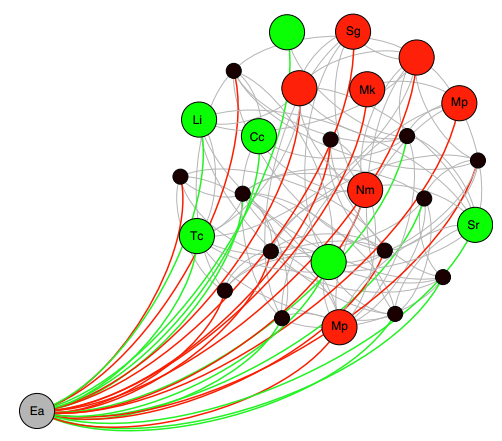
\includegraphics[scale=0.55]{jukush.png}
\caption{\textit{Erysiphe alphitoides} pathobiom on oak tree leaves.}
\end{figure}
\end{frame}

\begin{frame}{Data}
	\begin{itemize}
	\item \emphase{Species} : animal, bacteria, gene ...
	\item \emphase{Abundances} : ecological counts, Next-Generation Sequencing technologies...
	\item \emphase{Covariates} : coverage, temperature, water depth ... 
\end{itemize}
	Repeated signal : $n$ samples of $p$ abundances.
\pause
\begin{block}{Notations}
	$Y = [Y_{ij}]_{(i,j) \in \{1,...,n\} \times \{1,..., p\}} $
	\begin{itemize}
	\item $Y_{ij}$ : abundance of the $j^{th}$ species in the $i^{th}$ sample
\end{itemize}
\end{block}
\begin{center}
	\color{Nicered}{Infer the species interaction network from $Y$}
\end{center}
\end{frame}

\section{Network inference}
\subsection{Framework}
\begin{frame}{Graphical models}
	
\end{frame}
\subsection{Trees}
\section{Mixture tree}
%====================================================================
%====================================================================

\begin{frame}{Tree averaging} 
\tikzset{%
    observed/.style={%
    scale=0.6,circle,draw=Framableulight,transform shape,fill=white,font=\Large}
}
\begin{tabular}{p{.4\textwidth}}
 \begin{tabular}{ccccl}
   \begin{tabular}{c}
	\begin{tikzpicture}
		
      \tikzstyle{every edge}=[-,>=stealth',shorten >=1pt,auto,thin,draw]
    
		\node[observed] (Y1) at (0*\edgeunit, 0*\edgeunit) {$Y_1$};
		\node[observed] (Y2) at (1*\edgeunit, 0*\edgeunit) {$Y_2$};
		\node[observed] (Y3) at (1*\edgeunit, 1*\edgeunit) {$Y_3$};
		\node[observed] (Y4) at (0*\edgeunit, 1*\edgeunit) {$Y_4$};
		\path (Y1) edge [] (Y2)
        (Y1) edge [] (Y3)
        (Y2) edge [] (Y4);
   
	\end{tikzpicture}\\
	\footnotesize{$P\{T = T_1 | Y\}$}
	   \end{tabular}
	   & 
	   \hspace{-.05\textwidth} \pause
	   \begin{tabular}{c}
		\begin{tikzpicture}
		\tikzstyle{every observed}=[draw=none,text=black,scale=0.5,
      transform shape,circular drop shadow] 
		\node[observed] (Y1) at (0*\edgeunit, 0*\edgeunit) {$Y_1$};
		\node[observed] (Y2) at (1*\edgeunit, 0*\edgeunit) {$Y_2$};
		\node[observed] (Y3) at (1*\edgeunit, 1*\edgeunit) {$Y_3$};
		\node[observed] (Y4) at (0*\edgeunit, 1*\edgeunit) {$Y_4$};
		
		\path (Y1) edge [] (Y2)
        (Y1) edge [] (Y3)
        (Y1) edge [] (Y4);
		\end{tikzpicture} \\
		\footnotesize{$P\{T = T_2 | Y\}$}
	   \end{tabular}
	   &
	   \hspace{-.05\textwidth} \pause
	   \begin{tabular}{c}
		\begin{tikzpicture}
		\tikzstyle{every observed}=[draw=none,text=black,scale=0.5,
      transform shape,circular drop shadow] 
		\node[observed] (Y1) at (0*\edgeunit, 0*\edgeunit) {$Y_1$};
		\node[observed] (Y2) at (1*\edgeunit, 0*\edgeunit) {$Y_2$};
		\node[observed] (Y3) at (1*\edgeunit, 1*\edgeunit) {$Y_3$};
		\node[observed] (Y4) at (0*\edgeunit, 1*\edgeunit) {$Y_4$};
		
		\path (Y1) edge [] (Y2)
        (Y2) edge [] (Y3)
        (Y2) edge [] (Y4); 
		\end{tikzpicture}\\
		\footnotesize{$P\{T = T_3 | Y\}$}
	   \end{tabular}
	   &
	   \hspace{-.05\textwidth} \pause
	   \begin{tabular}{c}
		\begin{tikzpicture}
		\tikzstyle{every observed}=[draw=none,text=black,scale=0.5,
      transform shape,circular drop shadow] 
		\node[observed] (Y1) at (0*\edgeunit, 0*\edgeunit) {$Y_1$};
		\node[observed] (Y2) at (1*\edgeunit, 0*\edgeunit) {$Y_2$};
		\node[observed] (Y3) at (1*\edgeunit, 1*\edgeunit) {$Y_3$};
		\node[observed] (Y4) at (0*\edgeunit, 1*\edgeunit) {$Y_4$};
		 
		\path (Y1) edge [] (Y2)
        (Y3) edge [] (Y4)
        (Y2) edge [] (Y4);
		\end{tikzpicture} \\
		\footnotesize{$P\{T = T_4 | Y\}$}
	   \end{tabular}
	   & \hspace{-.06\textwidth} \huge{\emphase{...}}\normalsize   \\ \\
	   \\ \pause
	   \begin{tabular}{l}
		Compute edge\\
		probabilities:
	   \end{tabular}
	   &
	   \hspace{-.05\textwidth}
	   \begin{tabular}{c}
		\begin{tikzpicture}
		\node[observed] (Y1) at (0*\edgeunit, 0*\edgeunit) {$Y_1$};
		\node[observed] (Y2) at (1*\edgeunit, 0*\edgeunit) {$Y_2$};
		\node[observed] (Y3) at (1*\edgeunit, 1*\edgeunit) {$Y_3$};
		\node[observed] (Y4) at (0*\edgeunit, 1*\edgeunit) {$Y_4$};
		\draw [line width=5pt] (Y1) -- (Y2); 
		\draw [line width=3pt] (Y1) -- (Y3); 
		\draw [line width=.5pt] (Y1) -- (Y4); 
		\draw [line width=2pt] (Y2) -- (Y3); 
		\draw [line width=.5pt] (Y2) -- (Y4); 
 %		\draw [line width=.5pt] (Y3) -- (Y4); 
		\end{tikzpicture}\\
		\emphase{$P\{(j, k) \in T | Y\}$}
	   \end{tabular}
	   &
	   \hspace{-.05\textwidth} \pause
	   \begin{tabular}{l}
		Thresholding\\
		probabilities:
	   \end{tabular}
	   &
	   \hspace{-.05\textwidth}
	   \begin{tabular}{c}
		\begin{tikzpicture}
		\node[observed] (Y1) at (0*\edgeunit, 0*\edgeunit) {$Y_1$};
		\node[observed] (Y2) at (1*\edgeunit, 0*\edgeunit) {$Y_2$};
		\node[observed] (Y3) at (1*\edgeunit, 1*\edgeunit) {$Y_3$};
		\node[observed] (Y4) at (0*\edgeunit, 1*\edgeunit) {$Y_4$};
		\draw [line width=2pt] (Y1) -- (Y2); 
		\draw [line width=1.5pt] (Y1) -- (Y3); 
% 		\draw [line width=1pt] (Y1) -- (Y4); 
		\draw [line width=1pt] (Y2) -- (Y3); 
% 		\draw [line width=.1pt] (Y2) -- (Y4); 
% 		\draw [line width=1pt] (Y3) -- (Y4); 
		\end{tikzpicture}\\
		\emphase{$P\{(j, k) \in T | Y\}$}
	   \end{tabular}
	   &
	 \end{tabular}
    \end{tabular}
\end{frame}
%====================================================================
%====================================================================

\section{With count data}
\subsection{litterature}
\subsection{PLN}


\end{document}